\documentclass[border=5pt]{standalone}
\usepackage{tikz}
\usepackage{amsmath}
\usetikzlibrary{positioning, arrows.meta, calc, fit, backgrounds}

% --- Color Scheme (Warm Tones) ---
\definecolor{bgPrimary}{HTML}{FDEBD0}
\definecolor{bgSecondary}{HTML}{FAE5D3}
\definecolor{bgAccent}{HTML}{F5CBA7}
\definecolor{bgInput}{HTML}{FDF2E9}
\definecolor{borderPrimary}{HTML}{E59866}
\definecolor{borderAccent}{HTML}{CA6F1E}
\definecolor{arrowColor}{HTML}{A04000}
\definecolor{textMain}{HTML}{3E2723}
\definecolor{textLight}{HTML}{8D6E63}
\definecolor{bgHighlight}{HTML}{FADBD8}

% --- Styles ---
\tikzset{
  module/.style={
    draw=borderPrimary, fill=bgPrimary, rounded corners=4pt,
    minimum width=2.6cm, minimum height=1.2cm,
    font=\sffamily\small, text=textMain, line width=0.6pt, align=center,
  },
  novelmodule/.style={
    draw=borderAccent, fill=bgAccent, rounded corners=4pt,
    minimum width=2.6cm, minimum height=1.2cm,
    font=\sffamily\small\bfseries, text=textMain, line width=1.0pt, align=center,
  },
  iobox/.style={
    draw=borderPrimary, fill=bgInput, rounded corners=3pt,
    minimum width=2.0cm, minimum height=1.0cm,
    font=\sffamily\small, text=textMain, line width=0.5pt, align=center,
  },
  lossbox/.style={
    draw=borderAccent, fill=bgHighlight, rounded corners=3pt,
    minimum width=1.8cm, minimum height=0.7cm,
    font=\sffamily\footnotesize, text=textMain, line width=0.5pt, align=center,
  },
  stdarrow/.style={
    -{Stealth[length=5pt, width=4pt]}, line width=0.6pt, color=arrowColor,
  },
  lossarrow/.style={
    -{Stealth[length=4pt, width=3pt]}, line width=0.5pt, color=borderAccent, dashed,
  },
}

\begin{document}
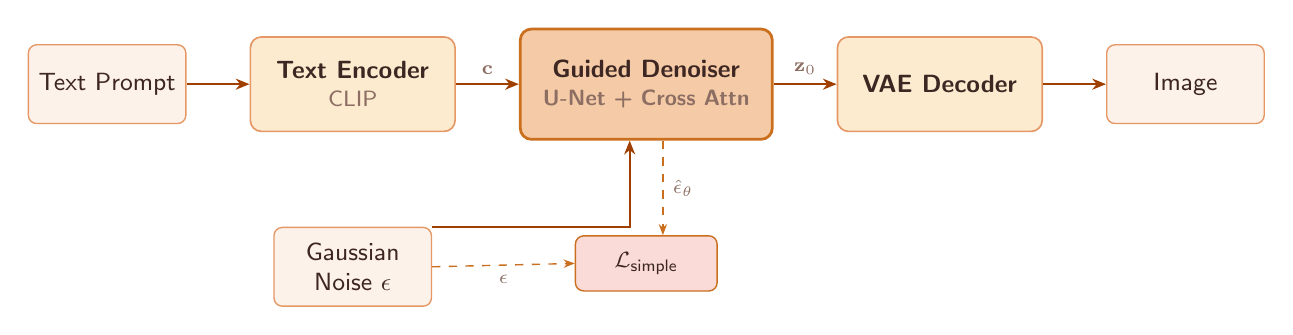
\begin{tikzpicture}

  % === Top row: forward diffusion (left to right) ===
  \node[iobox] (text) {Text Prompt};
  \node[module, right=0.8cm of text] (txtenc) {\textbf{Text Encoder}\\[-1pt]{\footnotesize\color{textLight}CLIP}};
  \node[novelmodule, right=0.8cm of txtenc, minimum width=3.2cm, minimum height=1.4cm] (denoise) {\textbf{Guided Denoiser}\\[-1pt]{\footnotesize\color{textLight}U-Net + Cross Attn}};
  \node[module, right=0.8cm of denoise] (vdec) {\textbf{VAE Decoder}};

  % === Output ===
  \node[iobox, right=0.8cm of vdec] (img) {Image};

  % === Bottom row: noise and loss ===
  \node[iobox, below=1.2cm of txtenc] (noise) {Gaussian\\Noise $\epsilon$};
  \node[lossbox, below=1.2cm of denoise] (loss) {$\mathcal{L}_{\text{simple}}$};

  % === Arrows: main pipeline ===
  \draw[stdarrow] (text) -- (txtenc);
  \draw[stdarrow] (txtenc) -- node[above, font=\sffamily\scriptsize, text=textLight] {$\mathbf{c}$} (denoise);
  \draw[stdarrow] (denoise) -- node[above, font=\sffamily\scriptsize, text=textLight] {$\mathbf{z}_0$} (vdec);
  \draw[stdarrow] (vdec) -- (img);

  % === Arrows: noise input ===
  \draw[stdarrow] (noise.north east) -| ([xshift=-6pt]denoise.south);

  % === Arrows: loss (predicted noise from denoiser + ground truth noise) ===
  \draw[lossarrow] ([xshift=6pt]denoise.south) -- node[right, font=\sffamily\scriptsize, text=textLight] {$\hat{\epsilon}_\theta$} ([xshift=6pt]loss.north);
  \draw[lossarrow] (noise.east) -- node[below, font=\sffamily\scriptsize, text=textLight] {$\epsilon$} (loss.west);

\end{tikzpicture}
\end{document}
